\chapter{Wstęp}

\section{Sztuczne sieci neuronowe}

Sztuczne sieci neuronowe mają obecnie bardzo mocno ugruntowaną pozycję szczególnie w dziedzinie problemów związanych z analizą i przetwarzaniem obrazów. Pomimo, iż nie jest to nowy pomysł, dopiero ostatni wzrost w wydajności komputerów pozwolił na ich praktyczne zastosowanie. Z matematycznego punktu widzenia są to sparametryzowane nieliniowe funkcje o pewnej ustalonej strukturze. Składają się z prostych elementów zwanych neuronami, a one natomiast są pogrupowane w warstwy. Połączenia między warstwami definiują przepływ danych. 'Nauka' sieci neuronowych polega na optymalizacji pewnej funkcji straty, czyli wyznaczeniu takich parametrów, żeby osiągnąć minimalny koszt. Do tego celu często korzysta się z metod opartych na SGD, a przy wybranej strukturze można w efektywny sposób zastosować algorytm propagacji wstecznej. W dalszej części pracy będę używał prostszej nazwy (neural nets). Przykładowa architektura sieci neuronowych jest zaprezentowana na wykresie \ref{fig:neural_nets}.

\begin{figure}[h!]
    \centering
    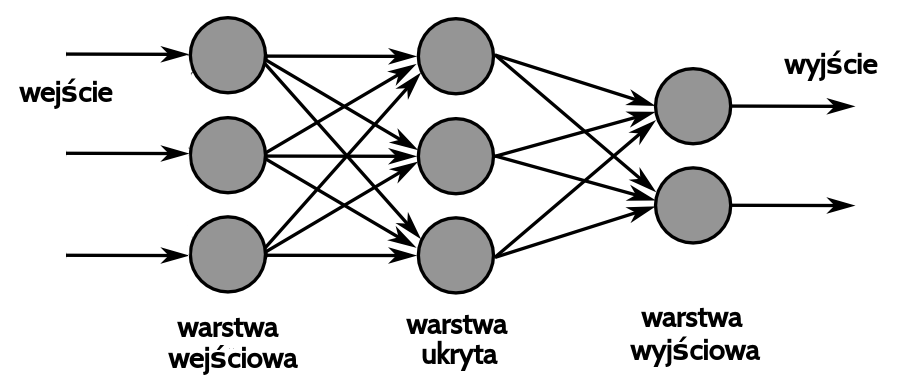
\includegraphics[width=0.6\textwidth]{images/neural_nets}
    \caption{Examplary architecture of the basic neural network}
    \label{fig:neural_nets}
\end{figure}

\section{Autoencoders}

Jest to jeden z rodzajów sieci neuronowych, służący do znajdowania wydajnej reprezentacji danych, co jest przykładem nauki bez nadzoru. W autoencoder'ach można wyróżnić dwie połączone ze sobą części: encoder i decoder. Zadaniem encodera jest wyprodukowanie reprezentacji, natomiast decoder służy do odtworzenia z niej oryginalnej postaci. Zależy nam na tym, żeby wyjście było w jakimś sensie jak najbardziej podobne do wejścia. W przypadku obrazów jako funkcja straty często stosowany jest błąd średnio kwadratowy (MSE). $Y _ { i }$ oznacza oryginalne dane, natomiast $\hat { Y } _ { i }$ zrekonstruowane.

$$
\mathrm { MSE } = \frac { 1 } { n } \sum _ { i = 1 } ^ { n } \left( Y _ { i } - \hat { Y } _ { i } \right) ^ { 2 }
$$

Przykładowy schemat znajduje się na wykresie \ref{fig:autoenc}. Zdjęcie kota zostaje włożone do encodera, a on znajduje jego liczbową reprezentację (czyli wektor o jakiejś ustalonej długości). Następnie tą reprezentacją karmiony jest dekoder, który ma za zadanie jak najlepiej odtworzyć oryginał. Chcemy mieć nadzieję, że taki model nauczy się dobrze układać wysoko wymiarowe dane w mniejszej przestrzeni, gdzie podobne do siebie obiekty będą blisko siebie. 

Często autoenkodery po wytrenowaniu nadają się do generowania całkiem nowych, nigdy jeszcze nie widzianych danych, ale podobnych do tych z zestawu uczącego. Można albo całkowicie wylosować wektor reprezentacji, albo delikatnie zmodyfikować dla już istniejącego przykładu. Dzięki temu możemy uzyskać realistycznie wyglądający obiekt o np. innym kolorze, kształcie. 

\begin{figure}[h!]
    \centering
    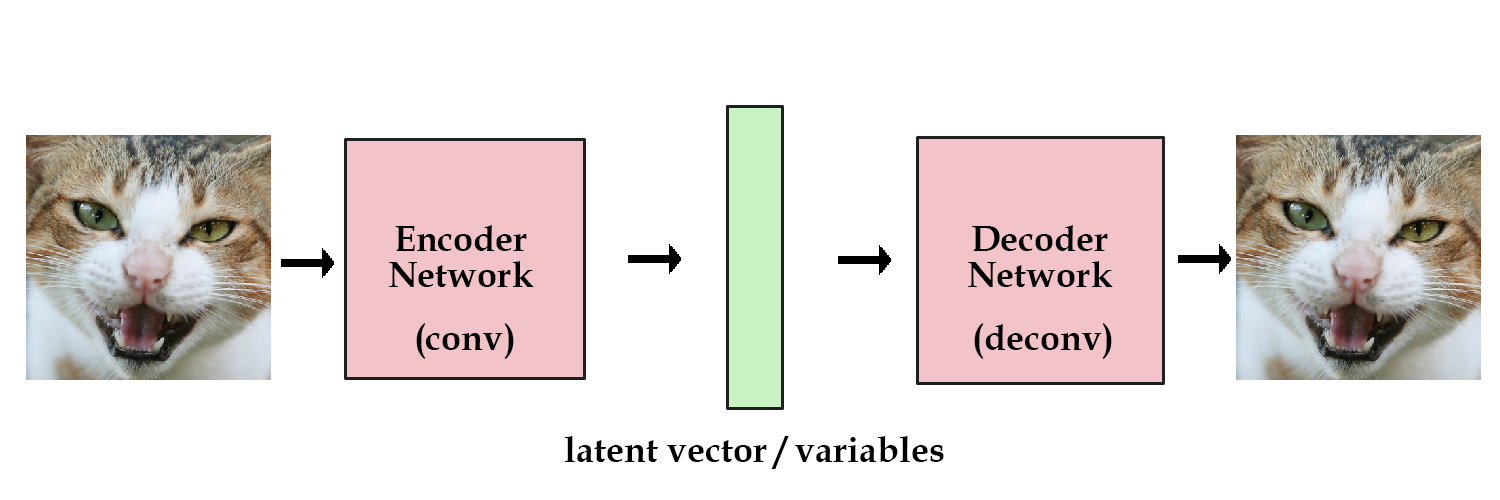
\includegraphics[width=1\textwidth]{images/autoenc}
    \caption{Architecture of autoencoder}
    \label{fig:autoenc}
\end{figure}

\section{Variational autoencoder}

W przypadku podstawowych autoenkoder'ów jednym z problemów jest brak kontroli nad tym jak dane są rozrzucane w przestrzeni. O ile sam model może bardzo dobrze rekonstruować dane, to same ich reprezentacja w przestrzeni może nie być ciągła, tj. pewne obszary nigdy nie były używane i dekoder nie za bardzo wie co zrobić, jeśli wylosujemy wektor z tego regionu. Jest to problemem przy generowaniu nowych danych, bądź interpolowaniu między nimi. W innych natomiast miejscach dane mogą zostać poukładane zbyt ciasno, co skutkować będzie błędną rekonstrukcją na niewidzianych danych. Próbą rozwiązania tych problemów jest właśnie Vaeriational Autoencoder.

Variational autoencoder rozszerza założenia o wprowadzenie modelowania rozkładu prawdopodobieństwa dla reprezentacji ukrytej. Czyli teraz encoder nie produkuje pojedyńczego wektora, ale dwa wektory interpretowane odpowiednio jako średnia $\mu$ oraz wariancja $\sigma$ dla rozkładu Gaussa. Następnie z tych parametrów formowany jest wektor, gdzie $i$-ty element powstał z $i$-tej pary $\mu$, $\sigma$.Dopiero taki wektor trafia do decodera, a z niego rekonstruowany jest wejściowa dana. Schemat przedstawiony jest na rysunku \ref{fig:vae_model}

Takie generowanie znaczy, że nawet dla tego samego wejścia i podczas gdy średnie oraz odchylenie zostaną takie same, to rzeczywiste kodowanie będzie się mimo wszystko różnić właśnie ze względu na to próbkowanie. 

\begin{figure}[h!]
    \centering
    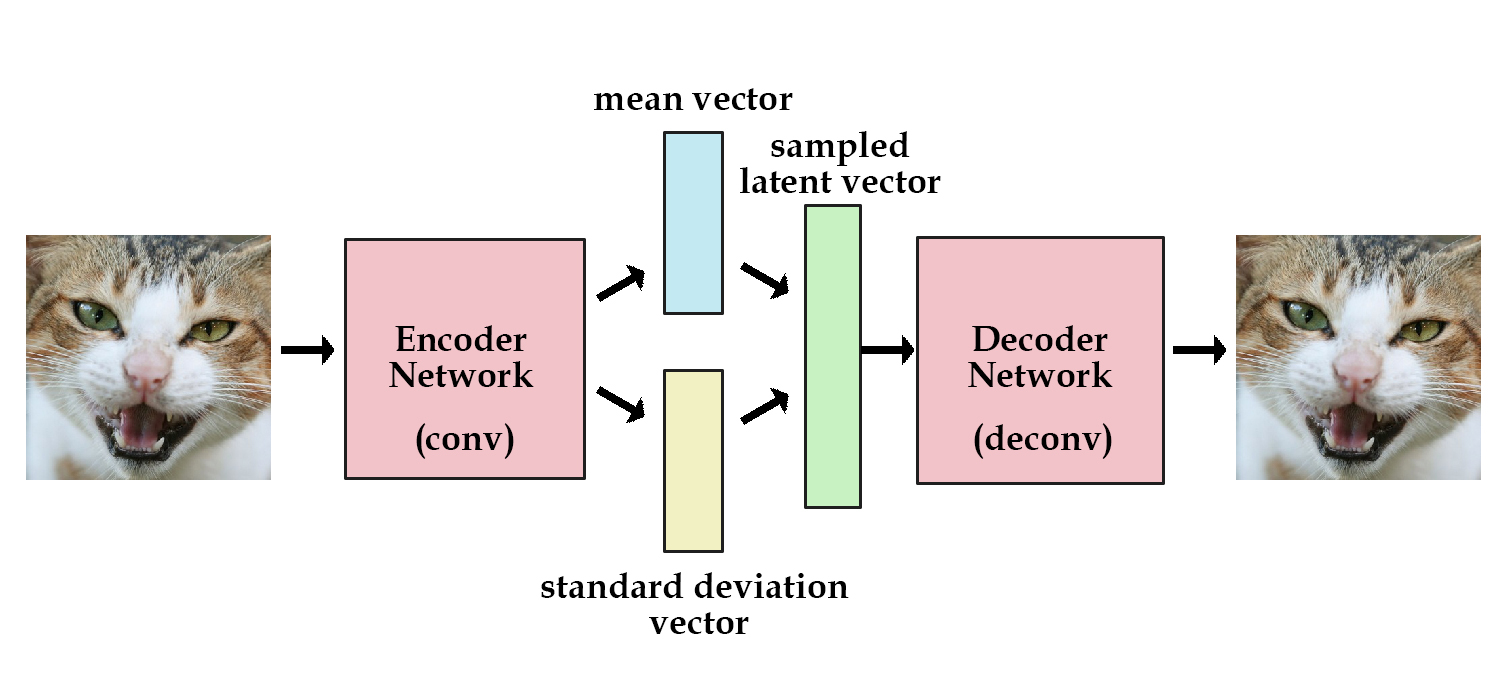
\includegraphics[width=1.0\textwidth]{images/vae_model}
    \caption{Architecture of Variational Autoencoder}
    \label{fig:vae_model}
\end{figure}

Intuicyjnie wektor średnich oznacza, gdzie zakodowana zmienna powinna być wycentrowana, natomiast odchylenie kontroluje obszar, wokół którego kodowanie może się różnić. Podczas gdy kodowanie jest losowane z wewnątrz koła, dekoder uczy się, że nie jedynie pojedynczy punkt z utajonej przestrzeni odnosi się do próbki, ale wszystkie punkty znajdujące się w pobliżu odnoszą się również do tego samego. To pozwala dekoderowi dekodować nie tylko pojedyncze, specyficzne reprezentacje (zostawiając przestrzeń nieciągłą), ale też te trochę się różniące, ponieważ narażony jest na szereg zmian kodowania tego samego wejścia podczas treningu. Rysunek \ref{fig:vae_vs_stand}

\begin{figure}[h!]
    \centering
    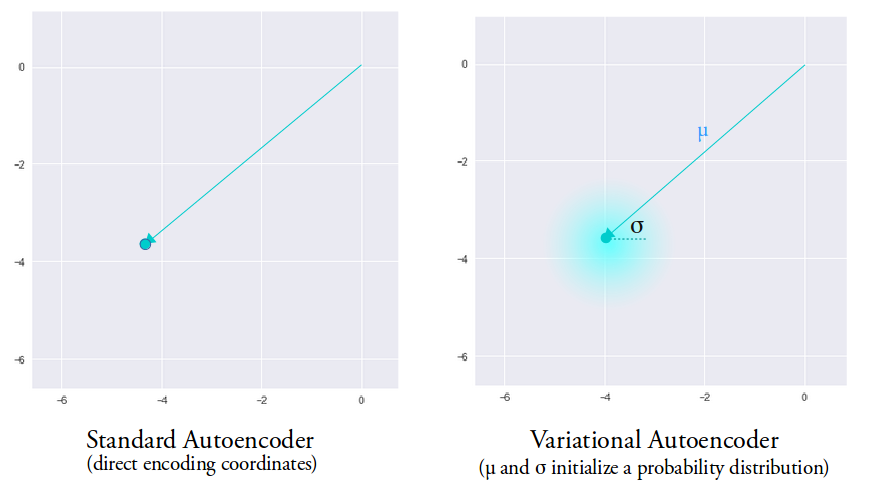
\includegraphics[width=0.7\textwidth]{images/vae_vs_stand}
    \caption{}
    \label{fig:vae_vs_stand}
\end{figure}

Model jest teraz wystawiony na pewien stopień lokalnej zmienności przez zmianę kodowania pojedynczej próbki, co skutkuje ciągłą przestrzenią w reprezentacji ukrytej dla lokalnego sąsiedztwa. Jednak na razie nie ma ograniczeń dla wartości jakie mogą przyjmować wektory $\mu$ i $\sigma$, przez co enkoder może nauczyć się generować bardzo różne $\mu$ dla różnych klas i grupować je minimalizując $\sigma$, upewniając się, że samo kodowanie nie różni się zbytnio dla tej samej próbki. W szczególności $\sigma$ może wynosić 0, przez co wrócimy do podstawowego modelu. To oczywiście pozwala dekoderowi na skuteczną rekonstrukcję, ale jedynie danych treningowych. Przykład przedstawiony jest na rysunku \ref{fig:vae_nolimits}. To co byśmy idealnie chcieli to kodowanie, gdzie grupy są blisko siebie, ale mimo wszystko są dobrze separowalne. Pozwoliłoby nam to na gładką interpolacje między próbkami i konstruowanie nowych danych.

\begin{figure}[h!]
    \centering
    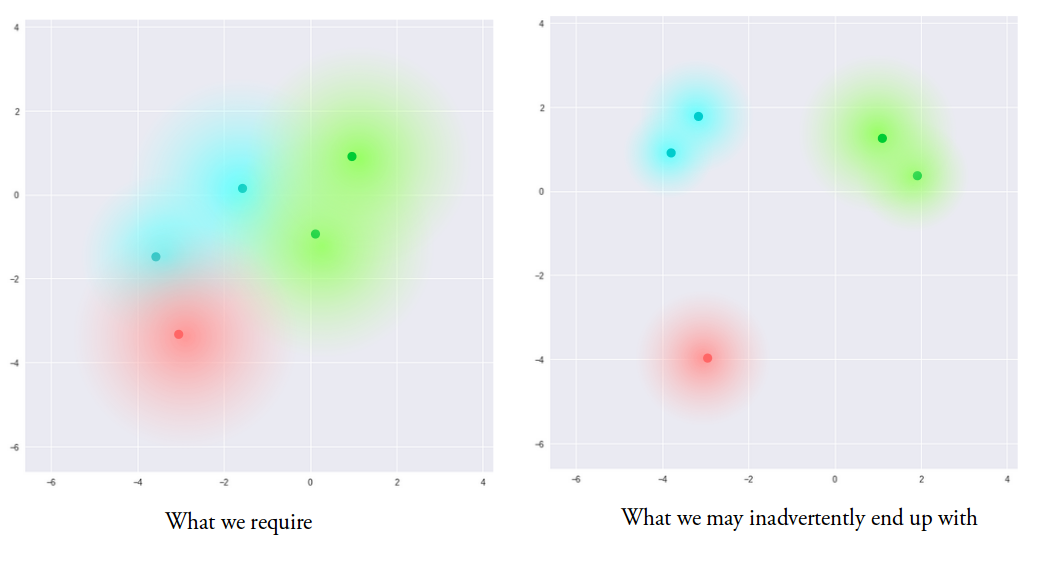
\includegraphics[width=0.7\textwidth]{images/vae_nolimits}
    \caption{Architecture of Variational Autoencoder}
    \label{fig:vae_nolimits}
\end{figure}

Żeby to osiągnąć wzbogacimy funkcję straty o koszt the Kullback–Leibler divergence. KL divergence mierzy po prostu różnicę pomiędzy dwoma rozkładami prawdopodobieństwa. Minimalizowanie go oznacza optymalizowania parametrów rozkładu ($\mu$ i $\sigma$), tak żeby jak najbardzieć przypominały celowy rozkład. W przypadku VAE będzie to standardowy rozkład normalny ($\mu = 0$,  $\sigma = 1$).

$$
\mathrm { KLD } = \sum _ { i = 1 } ^ { n } \sigma _ { i } ^ { 2 } + \mu _ { i } ^ { 2 } - \log \left( \sigma _ { i } \right) - 1
$$

\subsection{Magia, która za tym stoi}

To co do tej pory napisałem to były w większości intuicje i nasze zachcianki. Chciałbym teraz przedstawić jak to wygląda od strony matematycznej.

\add[inline]{Dokończyć matmę}

%\section{Convolutional VAE}
%
%Jest to rozszerzenie poprzedniego modelu, w którym dodatkowo stosujemy warstwy splotowe. Szczególnie w przypadku obrazów pozwala to na zwiększenie rozmiaru danych wejściowych przez zmniejszenie ilości parametrów w stosunku do warstw fully-connected oraz wykryciu na wstępie jakiś prostych cech, przez co w reprezentacji mogą znajdowac się bardziej abstrakcyjne rzeczy. 

\section{Deep feature consistent variational auto-encoder}

W autoenkoderze wariacyjnym jednym ze składników kosztu jest błąd rekonstrukcji. Standardowo funkcja ta oparta jest na porównywaniu wartości odpowiadającym sobie pikselom z oryginalnego obrazu i tego zrekonstruowanego. Często przyczynia się to do uśredniania wartości pikseli przez co wyjściowy obraz nie jest wyraźny. Przyczynie sie do tego między innymi fakt, że taki liczenie błędu jest bardzo czułe na chociażby przesunięcie. Oryginalny obraz i ten lekko przesunięty mimo, iż nie różnią się prawie wogóle perceptualnie dla człowieka, to ich koszt MSE jest bardzo duży. Uśrednianie wartości jest sposobem na optymalizowanie tego problemu. Wynika z tego, że raczej chcielibyśmy patrzeć na to co znajduje się na obrazkach, niż porównywać poszczególne piksele.

I w tym właśnie miejscu pojawia się Deep feature consistent. Opiera się ona na wykorzystaniu wcześniej już wyuczonej sieci splotowej. W takich sieciach coraz głębsze filtry odpowiadają za rozpoznawanie coraz to bardziej abstrakcyjnych cech. Będziemy teraz myśleć, że dwa obrazy są podobne, jeśli maja podobne wartości aktywacji w warstwach ukrytych tej sieci. Dzięki takiemu patrzeniu na różnice dwa obrazy powinny być podobne nawet jeśli zostaną poddane takim operacjom jak m.in przesunięcie, rotacja, co stanowi duży problem dla kosztów typu pixel-to-pixel. Bład ten jest okreslany mianem perceptual loss.

\begin{figure}[h!]
    \centering
    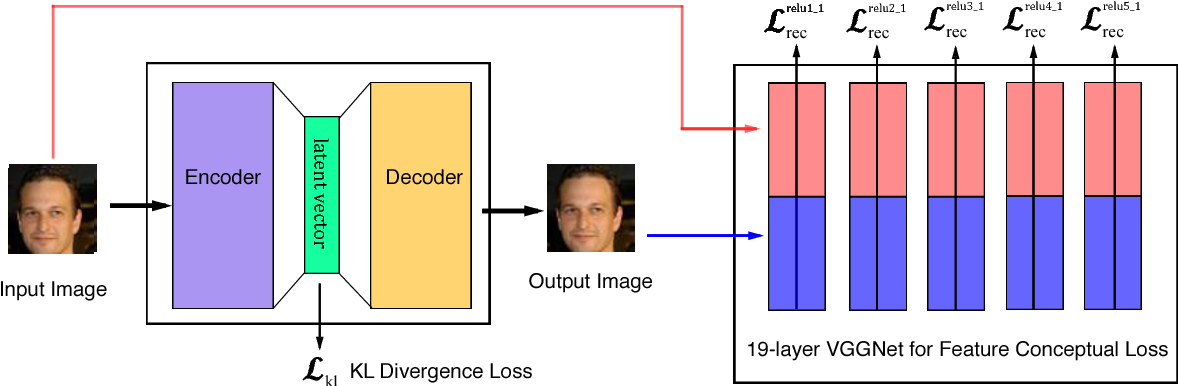
\includegraphics[width=0.8\textwidth]{images/dfc_vae}
    \caption{Architecture of Variational Autoencoder}
    \label{fig:dfc_vae}
\end{figure}
